
\documentclass[border=4pt]{standalone}
\usepackage[utf8]{inputenc}
\usepackage[T1]{fontenc}
\usepackage{amsmath,amssymb,xcolor}
\usepackage{tikz}
\usetikzlibrary{arrows.meta,shapes.misc}
\renewcommand{\familydefault}{\sfdefault}
\definecolor{vbleu}{HTML}{1C5FD6}
\definecolor{orange}{HTML}{E8590C}
\definecolor{vert}{HTML}{2F9E44}
\definecolor{gris}{HTML}{495057}
\definecolor{violet}{HTML}{7048E8}
\tikzset{
  vec/.style={->,very thick,>={Stealth[length=2.4mm]}},
  ref/.style={orange,thick,dashed},
  par/.style={vert,thick,dashed},
  sec/.style={gris,thick,dashed},
  ptcross/.style={cross out,draw,thick,minimum size=1.6mm,inner sep=0pt},
}
\usepackage{array}
\setlength{\parindent}{0pt}\setlength{\parskip}{5pt}
\newcommand{\V}[1]{\overrightarrow{\mathrm{#1}}}
\begin{document}

\begin{minipage}{16cm}\large \colorbox{vert!8}{\begin{minipage}{15.5cm}\vspace{4pt}{\color{vert}Définition 7 — \textit{Vecteurs colinéaires}}\par Deux vecteurs $\vec{u}$ et $\vec{v}$ sont dits {\color{vert}colinéaires} s'il existe un réel $k$ tel que $\vec{v}=k\,\vec{u}$ ou $\vec{u}=k\,\vec{v}$.\par Le réel $k$ est appelé {\color{vert}coefficient de colinéarité}.\vspace{4pt}\end{minipage}}\par\vspace{8pt}\colorbox{gray!10}{\begin{minipage}{15.5cm}\vspace{4pt}{\color{gris}Exemple}\par \begin{minipage}[c]{6.6cm}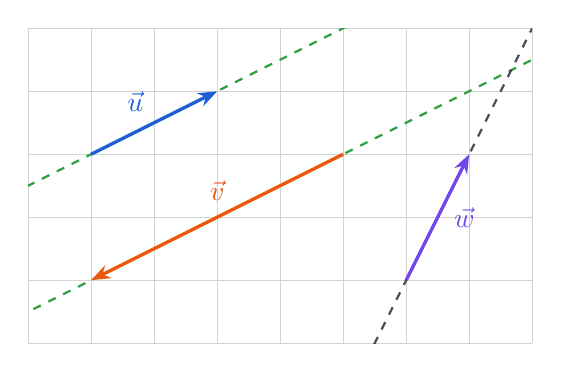
\begin{tikzpicture}[x=0.8cm,y=0.8cm]
\draw[gray!35,thin,step=0.8cm] (0,0) grid (8,5);
\begin{scope}\clip (0,0) rectangle (8,5);
\draw[par] (-79,-37) -- (81,43);
\draw[par] (165,83) -- (-155,-77);
\draw[sec] (-34,-79) -- (46,81);
\end{scope}
\draw[vec,vbleu] (1,3) -- (3,4) node[midway,above left] {$\vec{u}$};
\draw[vec,orange] (5,3) -- (1,1) node[midway,above=2pt] {$\vec{v}$};
\draw[vec,violet] (6,1) -- (7,3) node[midway,right=2pt] {$\vec{w}$};
\end{tikzpicture}\end{minipage}\hspace{0.4cm}\begin{minipage}[c]{8.4cm}Les droites qui portent $\vec{u}$ et $\vec{v}$ (pointillés verts) sont parallèles : $\vec{u}$ et $\vec{v}$ ont la même direction.\\ On a $\vec{v}=-2\,\vec{u}$. Donc $\vec{u}$ et $\vec{v}$ sont colinéaires.\\ Le coefficient de colinéarité est $-2$.\par La droite qui porte $\vec{w}$ (pointillés gris) est sécante avec les deux autres.\\ Donc $\vec{w}$ n'est colinéaire ni à $\vec{u}$, ni à $\vec{v}$.\end{minipage}\vspace{4pt}\end{minipage}}\end{minipage}
\end{document}
